\documentclass[journal,5pt,twocolumn]{IEEEtran}
%\makeatletter
\usepackage{tikz}
\usepackage[siunitx]{circuitikz}
\usetikzlibrary{shapes,arrows}
\makeatother
\usepackage{setspace}
\usepackage{gensymb}
\usepackage{xcolor}
\usepackage{caption}
%\usepackage{stackengine}
%\usepackage{subcaption}
%\doublespacing
\usepackage{xcolor}
\usepackage{lipsum}
\singlespacing
\def\baselinestretch{1.5}
\usepackage{fancyhdr}
\pagestyle{fancy}
\fancyhf{} 

%\counterwithin{enumi}{section}
%\counterwithin{equation}{enumi}
%\counterwithin{figure}{enumi}

\newcommand\figref{Fig.~\ref}
\usepackage[colorlinks=true, allcolors=black]{hyperref}

\usepackage{graphicx}
%\graphicspath{ {./images}  }
%\usepackage{amssymb}
%\usepackage{relsize}
\usepackage[cmex10]{amsmath}
\usepackage{mathtools}
%\usepackage{amsthm}
\interdisplaylinepenalty=2500
%\savesymbol{iint}
%\usepackage{txfonts}
%\restoresymbol{TXF}{iint}
\usepackage{wasysym}
\usepackage{amsthm}
\usepackage{mathrsfs}
\usepackage{txfonts}
\usepackage{stfloats}
\usepackage{cite}
\usepackage{cases}
\usepackage{mathtools}
\usepackage{subfig}
\usepackage{enumerate}	
\usepackage{enumitem}
\usepackage{amsmath}
\usepackage{circuitikz}
\usepackage{longtable}
\usepackage{multirow}
%\usepackage{algorithm}
%\usepackage{algpseudocode}
\usepackage{enumitem}
\usepackage{mathtools}
\usepackage{tikz}
\usetikzlibrary{shapes,arrows,automata,petri,positioning,calc}
%\usetikzlibrary{arrows.meta,calc,positioning}
%\usepackage[framemethod=tikz]{mdframed}
\usepackage{listings}
    \usepackage[latin1]{inputenc}                                 %%
    \usepackage{color}                                            %%
    \usepackage{array}                                            %%
    \usepackage{longtable}                                        %%
    \usepackage{calc}                                             %%
    \usepackage{multirow}                                         %%
    \usepackage{hhline}                                           %%
    \usepackage{ifthen}                                           %%
  %optionally (for landscape tables embedded in another document): %%
    \usepackage{lscape}     


%\usepackage{stmaryrd}


%\usepackage{wasysym}
%\newcounter{MYtempeqncnt}
\DeclareMathOperator*{\Res}{Res}
%\renewcommand{\baselinestretch}{4}
%\setcounter{secnumdepth}{4}
\renewcommand\thesection{\arabic{section}}
\renewcommand\thesubsection{\thesection.\arabic{subsection}}
\renewcommand\thesubsubsection{\thesubsection.\arabic{subsubsection}}

\hyphenation{Future Wireless communications}

%\lstset{
%language=C,
%frame=single, 
%breaklines=true
%}

\def\inputGnumericTable{}                                 %%

\lstset{
%language=python,
frame=single, 
breaklines=true,
columns=fullflexible
}

 \usepackage{watermark}

\begin{document}
%
\tikzstyle{block} = [rectangle, draw,
text width=7em, text centered, minimum height=4em]
\tikzstyle{sum} = [draw, circle, node distance=3cm]
\tikzstyle{input} = [coordinate]
\tikzstyle{output} = [coordinate]
\tikzstyle{pinstyle} = [pin edge={to-,thin,black}]
\tikzstyle{line} = [draw, -latex']
\theoremstyle{definition}
\newtheorem{theorem}{Theorem}[section]
\newtheorem{problem}{Problem}
\newtheorem{proposition}{Proposition}[section]
\newtheorem{lemma}{Lemma}[section]
\newtheorem{corollary}[theorem]{Corollary}
\newtheorem{example}{Example}[section]
\newtheorem{definition}{Definition}[section]
%\newtheorem{algorithm}{Algorithm}[section]
%\newtheorem{cor}{Corollary}
\newcommand{\BEQA}{\begin{eqnarray}}
\newcommand{\EEQA}{\end{eqnarray}}
\newcommand{\define}{\stackrel{\triangle}{=}}
\bibliographystyle{IEEEtran}
%\bibliographystyle{ieeetr}
\providecommand{\nCr}[2]{\,^{#1}C_{#2}} % nCr
\providecommand{\nPr}[2]{\,^{#1}P_{#2}} % nPr
\providecommand{\mbf}{\mathbf}
\providecommand{\pr}[1]{\ensuremath{\Pr\left(#1\right)}}
\providecommand{\qfunc}[1]{\ensuremath{Q\left(#1\right)}}
\providecommand{\sbrak}[1]{\ensuremath{{}\left[#1\right]}}
\providecommand{\lsbrak}[1]{\ensuremath{{}\left[#1\right.}}
\providecommand{\rsbrak}[1]{\ensuremath{{}\left.#1\right]}}
\providecommand{\brak}[1]{\ensuremath{\left(#1\right)}}
\providecommand{\lbrak}[1]{\ensuremath{\left(#1\right.}}
\providecommand{\rbrak}[1]{\ensuremath{\left.#1\right)}}
\providecommand{\cbrak}[1]{\ensuremath{\left\{#1\right\}}}
\providecommand{\lcbrak}[1]{\ensuremath{\left\{#1\right.}}
\providecommand{\rcbrak}[1]{\ensuremath{\left.#1\right\}}}
\theoremstyle{remark}
\newtheorem{rem}{Remark}
\newcommand{\sgn}{\mathop{\mathrm{sgn}}}
\providecommand{\abs}[1]{\left\vert#1\right\vert}
\providecommand{\res}[1]{\Res\displaylimits_{#1}} 
\providecommand{\norm}[1]{\lVert#1\rVert}
\providecommand{\mtx}[1]{\mathbf{#1}}
\providecommand{\mean}[1]{E\left[ #1 \right]}
\providecommand{\fourier}{\overset{\mathcal{F}}{ \rightleftharpoons}}
%\providecommand{\hilbert}{\overset{\mathcal{H}}{ \rightleftharpoons}}
\providecommand{\system}{\overset{\mathcal{H}}{ \longleftrightarrow}}
	%\newcommand{\solution}[2]{\textbf{Solution:}{#1}}
\newcommand{\solution}{\noindent \textbf{Solution: }}
\newcommand{\myvec}[1]{\ensuremath{\begin{pmatrix}#1\end{pmatrix}}}
\providecommand{\dec}[2]{\ensuremath{\overset{#1}{\underset{#2}{\gtrless}}}}
\DeclarePairedDelimiter{\ceil}{\lceil}{\rceil}
%\numberwithin{equation}{subsection}
\numberwithin{equation}{section}
%\numberwithin{problem}{subsection}
%\numberwithin{definition}{subsection}
%\makeatletter
%\@addtoreset{figure}{section}
%\makeatother
\let\StandardTheFigure\thefigure
%\renewcommand{\thefigure}{\theproblem.\arabic{figure}}
%\renewcommand{\thefigure}{\thesection}
%\numberwithin{figure}{subsection}
%\numberwithin{equation}{subsection}
%\numberwithin{equation}{section}
%\numberwithin{equation}{problem}
%\numberwithin{problem}{subsection}
%\numberwithin{problem}{section}
%%\numberwithin{definition}{subsection}
%\makeatletter
%\@addtoreset{figure}{problem}
%\makeatother
%\makeatletter
%\@addtoreset{table}{problem}
%\makeatother
\let\StandardTheFigure\thefigure
\let\StandardTheTable\thetable
\let\vec\mathbf
%%\renewcommand{\thefigure}{\theproblem.\arabic{figure}}
%\renewcommand{\thefigure}{\theproblem}
%%\numberwithin{figure}{section}
%%\numberwithin{figure}{subsection}
\def\putbox#1#2#3{\makebox[0in][l]{\makebox[#1][l]{}\raisebox{\baselineskip}[0in][0in]{\raisebox{#2}[0in][0in]{#3}}}}
     \def\rightbox#1{\makebox[0in][r]{#1}}
     \def\centbox#1{\makebox[0in]{#1}}
     \def\topbox#1{\raisebox{-\baselineskip}[0in][0in]{#1}}
     \def\midbox#1{\raisebox{-0.5\baselineskip}[0in][0in]{#1}}
\title{ 
%	\logo{
FREQUENCY MODULATION
%	}
}
\author{ Under guidance of Dr. GVV SHARMA}% <-this % stops a space
%\thiswatermark{\centering \put(-50,-105){%\includegraphics[scale=1]{iith.png}}} 
% make the title area
\maketitle
\tableofcontents
\section{\textbf{Introduction}}
Frequency modulation (FM) is a widely used technique in modern communication systems. It is a form of modulation that encodes information by varying the frequency of a carrier signal in proportion to the message signal\\
One important parameter in FM is the bandwidth, which determines the range of frequencies required to accurately represent the modulated signal. The Carson's rule provides a simple approximation for the bandwidth of an FM signal.In this the bandwidth of an FM signal can be calculated by analyzing its frequency spectrum using techniques such as Fourier analysis.
\section{\textbf{Generating FM:}}
\subsection{\textbf{Bandwidth calculation method}}

Bandwidth refers to the range of frequencies over which a signal or system operates. There are several methods to calculate the bandwidth of a signal, including the 3dB attenuation method and the spectral density method.\\
\begin{enumerate}
\item  The 3dB attenuation method involves finding the frequency range where the signal's power or amplitude is reduced by half (-3dB) from its maximum value.However, it does not take into account the full frequency spectrum of the signal or system, and may not accurately reflect the actual bandwidth of the signal.

\item The spectral density method calculates the bandwidth of a signal or system by analyzing its frequency content. Specifically, it calculates the power spectral density (PSD) of the signal or system, which is a measure of how the power of the signal is distributed across different frequencies. The bandwidth is then defined as the frequency range over which 99\%of the total power is contained.\\
 This method provides a more accurate and comprehensive measure of bandwidth as it takes into account the entire frequency spectrum of the signal or system.
\end{enumerate}

\subsection{\textbf{Steps for calculating the bandwidth of the signal}}
   

\begin{enumerate}
\item Loading the Audio File:  Load the WAV file containing the audio input signal.
The audio input signal is a time-varying signal, and we need to convert it into the frequency domain to analyze its bandwidth.



\item Computing the Fourier Transform:

To plot the spectrum of the message signal, we need to compute the Fourier Transform of the message signal, which will give us the frequency domain representation of the signal.

\begin{equation}
M_k = \sum_{n=0}^{N-1} m(n) e^{-j2\pi kn/N}, \quad k=0,1,\dots,N-1
\end{equation}
In code for computing the FFT of m(n)
\begin{equation}
M_k = \texttt{fft}(x(n), N)
\end{equation}
The spectrum of input audio signal is plotted in \figref{fig:input_spectrum}
\begin{figure}
\centering 
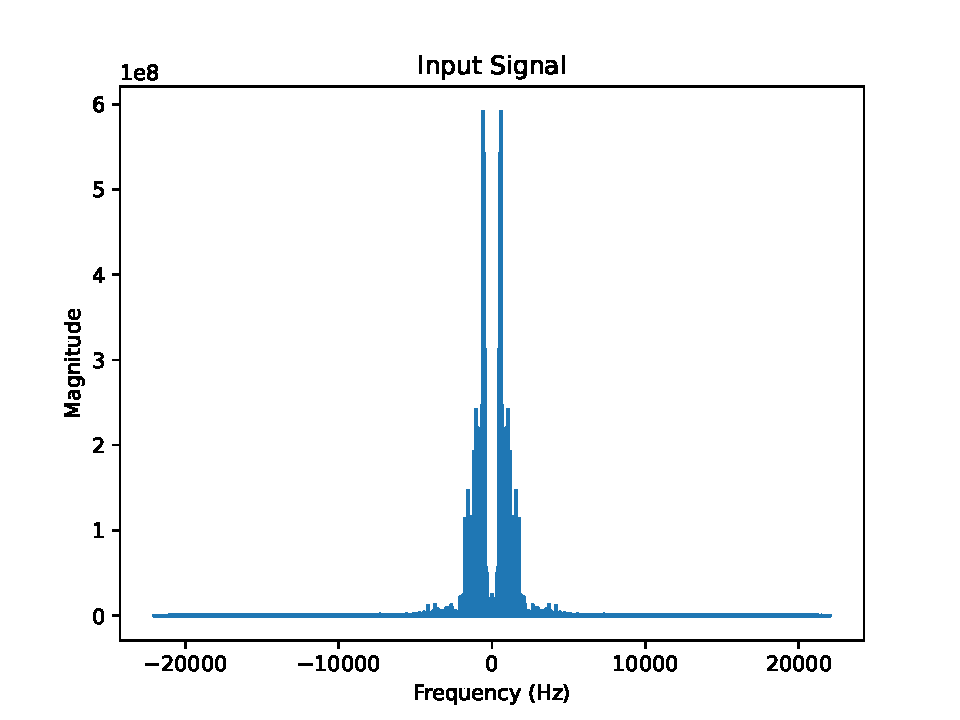
\includegraphics[width=\columnwidth]{inputs.pdf} 
\caption{spectrum analysis of input signal}
\label{fig:input_spectrum}
\end{figure}

\iffalse
\begin{align*}
M(f) = FFT(m(t))
\end{align*}
Where M(f) is the frequency representation of the signal, m(t) is the input signal
\fi
\item Calculating the frequency Range: Calculates the frequencies for each sample in the audio signal. The frequency range is used to plot the magnitude spectrum of the audio signal.

\item Calculating the Power Spectral Density:
\begin{align*}
PSD(f)=\lvert M(f) \rvert^2 
\end{align*}
Where PSD(f) is the power spectral density at frequency f, M(f) is the Fourier Transform of the input signal

\item Finding the Frequency Range with Significant Power:
The frequency range with significant power in the PSD of the FM signal. This can be done by creating a mask that identifies frequencies where the PSD is greater than a certain threshold. Then the mask can be defined as:

\iffalse
\begin{align*}
mask(f) &=
\begin{cases}
 PSD(f) \quad PSD(f) > T\\
0 \quad otherwise
\end{cases}
\end{align*}
\fi
\begin{align*}
mask(f) = 
    \begin{cases}
        True \quad \text{if } fm\_psd(f) > 0.1 * \max(fm\_psd) \\
        False \quad \text{if } fm\_psd(f) \leq 0.1 * \max(fm\_psd)
    \end{cases}
\end{align*}

python code  :\\
\begin{lstlisting}
# Find frequency range with significant power of FM signal
fm_mask = fm_psd > 0.1*np.max(fm_psd)
fm_freq_range = fm_freqs[fm_mask]
fm_bandwidth = max(fm_freq_range) - min(fm_freq_range)
print('FM Bandwidth:', fm_bandwidth, 'Hz')
\end{lstlisting}






\begin{tabular}{|c|l|c|}
    \hline 
    \textbf{Parameter} & \textbf{Value} &\textbf{Description} \\ \hline
    T&0.1&Threshold\\
    $F_s$ & 44100 Hz & Sampling rate\\ 
    t     & 22 $\mu$ & Sampling time\\  \hline
    \end{tabular}
\vspace{10mm}
\item Calculating the Bandwidth: The bandwidth can be calculated mathematically using the following formula:
\begin{align*}
B=mask_{maxi}-mask_{min}
\end{align*}
where $mask_{maxi}$ and $mask_{min} $ are themaximum amd minimum frequency bounds of the range  respectively.\\
Analyzes the audio signal and plots its magnitude spectrum. The bandwidth of the audio signal is  calculated using power spectral density. Obtain the bandwidth of the audio as 2 khz using below code
\begin{center}
\fcolorbox{red}{white}{\parbox{7.5cm}
{\href{https://github.com/KrishnaYadati/signal-processing/tree/main/fm/codes/input.py}
{/codes/input.py}}}
\end{center}
\end{enumerate}
\section{\textbf{Modulation:}}
\begin{figure}
\hspace{-1.2cm} 
\begin{circuitikz} [scale=.73,font=\footnotesize]

%\draw (5,5) -- (6.5,5) to[R=$R_4:47k\Omega$, label=$\mathrm{R_4}$, left] (6.5,2);

\draw (0,0) node[circ] {} to[C=$C_1$] node[pos=0.07,below left=1.5ex]{\SI{0.1}{\mu F}} ++(3.7,0) node[npn, anchor=B] (Q1) {$Q_1$};
\draw(4.85,-0.5)--(4.85,-4);
%\draw (0,0) -- (0,5) to[R=$R_3 47k\Omega$](5,5);
\draw (0,0)--(0,5) to[R=$R_3$]  node[pos=0.05,below left=1.5ex]{\SI{47}{k\Omega}}(5,5);
\draw (3,0)--(3,2) to[R=$R_1$]  node[pos=0.05,below left=1.5ex]{\SI{1}{M\Omega}}(4.85,2)--(4.85,.5);
\draw (4.8,2)--(5,2) to[C=$C_2$]node[pos=1.8,below left=1.2ex]{\SI{0.1}{\mu F}} (6.5,2);
%\draw(4.85,2)--(4.85,2.5) to[R=$R_2:10k\Omega$](4.85,5);
\draw (4.85,2)--(4.85,2.5) to[R=$R_2$]  node[pos=0.15,below left=1ex]{\SI{10}{k\Omega}}(4.85,5);
\draw (5,5) -- (6.5,5) to[ R]node[pos=-1.5,above left]{$R_4$} node[pos=-0.8,above left=1ex]{\SI{47}{k\Omega}} (6.5,2);
%\draw (5,5) -- (6.5,5) to[R=$R_4$]node[pos=0.1,above right=1ex]{\SI{47}{k\Omega}}(6.5,2);
\draw (6.5,2)--(6.5,-2) to[C=$C_3$] node[pos=-0.01,above left=1.5ex]{\SI{1}{ nF}} (6.5,-4);
\draw (0,0)--(0,-2) to [mic]node[pos=0.08,above right=2ex]{mic}(0,-4);
\draw(6.5,5)--(9,5);
\draw (9,5)--(9,4.5);

\draw(9,4.5)--(7.5,4.5)to[C=$C_6$]node[pos=0.01,above right=1.5ex]{\SI{33}{pF}} (7.5,2.5);
 %\draw(9,4.5)--(7.75,4.5)to[C]node[pos=-1.2,above left]{$C_6$} node[pos=-0.5,above left=1ex]{\SI{33}{pF}} (7.75,2.5);
\draw(9,4.5)to[C=$C_5$]node[pos=0.01,above right=1.5ex]{\SI{33}{pF}} (9,2.5);
\draw(7.5,4.5)--(10.5,4.5)to[L=$L_1$] node[pos=1.2,above right=2.5ex]{\SI{1}{\mu H}} (10.5,2.5);
\draw (7.5,2.5)--(10.5,2.5);
\draw(9,2.5)to[C=$C_4$] node[pos=0.01,below right=1.5ex]{\SI{10}{pF}} (9,-1.5);
\draw(9,-1.5)--(7.75,-1.5);
\draw(6.5,0)--(6.6,0);
\draw(0,0) ++(6.6,0) node[npn, anchor=B] (Q2){$Q_2$};
\draw(7.74,.5)--(7.74,1.5)--(9,1.5);
\draw(7.74,-0.5)--(7.74,-1.5);
\draw(7.74,-1.5)to[R=$R_5\ 470\Omega$] (7.74,-4);
\draw(9,1.5)--(9.75,1.5)to[C=$C_7$]node[pos=0.01,below right=1.5ex]{\SI{10}{pF}}  (10,1.5);
\draw(10,1.5)--(11,1.5);
\draw(11,1.5)--(11,2.5) node[antenna] {antenna};
\draw(9,5)--(12.5,5)to[C=$C_8$] node[pos=0.01,below right=1.5ex]{\SI{0.1}{\mu F}}(12.5,-4);
\draw(12.5,5)--(14.5,5)to[battery,l=\SI{12}{\V}](14.5,-4);
\draw(0,-4)--(14.5,-4);
\end{circuitikz}
\captionof{figure}{FM Transmitter Circuit}
\label{fig:tx_cir}
\end{figure} 



  
  \begin{table}[h]
\centering
\begin{tabular}{|l|c|r|}
\hline
\textbf{Component} & \textbf{Quantity} & \textbf{Value} \\ \hline
Transistor & 2 & 2N3904 \\ \hline
Inductor &1&1 $\mu$H \\ \hline
Resistor & 1 & 1M \\ 
& 1 & 470$\Omega$ \\ 
& 2 & 47k$\Omega$ \\ 
& 1 & 10k$\Omega$ \\ \hline
Capacitor & 1 & 1nF \\ 
& 3 & 0.1$\mu$F \\ 
& 2 & 10pF \\ 
& 2 & 33pF \\ \hline
Condenser mic & 1 & \\ \hline
Antenna & 1& \\ \hline
\end{tabular}
\caption{List of components}
\label{tab:components}
\end{table}

\begin{figure}
\tikzstyle{block} = [rectangle, draw, fill=white!20, text width=6em, text centered, rounded corners, minimum height=4em]
\tikzstyle{line} = [draw, -latex']

\begin{tikzpicture}[node distance=3cm, auto]
    % block
    \node [block] (audio) {$m(t)$ };
   
    \node [block, above of=audio ] (int) {integrator};
     \node [block, right of=int] (kf) {2$\pi$K$_f$};
%\node[circle, draw, state, accepting, right of=kf] (sum) {$\sum$};
      \node [block, right of=kf ] (sum) {Phase Modulator};
    \node [block, above of=sum ] (carrier) {$A_c$cos(2$\pi$f$_{c}$t)};
   \node [block, below of=sum ] (fm){$A_c \cos (2 \pi F_c t$ \\$+ 2\pi K_{f}$\\ $ \int_{0}^t m(\tau) d\tau )$ };
    
    
    % lines
    \path [line] (audio) -- (int);
    \path [line] (int) -- (kf);
    \path [line] (kf) -- (sum);
    \path [line] (carrier) -- (sum);
     \path [line] (sum) -- (fm);
    
    
\end{tikzpicture}
\captionof{figure}{FM Transmitter Block Diagram }
\label{fig:tx_blk}
\end{figure}
\begin{enumerate}
 \item Frequency modulation to the sound signal:


 \begin{equation}
 c(t) = A_c \cos(2 \pi F_c t )
 \label{eq:carrier_signal} 
 \end{equation}
 Equation \ref{eq:carrier_signal} shows the mathematical expression for a carrier signal with amplitude $A_c$, frequency $F_c$. 
 
 The frequency modulation is applied to the sound signal using the formula
 \begin{equation}
 s(t) = A_c \cos \left(2 \pi F_c t +2\pi K_{f} \int_{0}^t m(\tau) d\tau \right) 
 \end{equation}

 where $A_c$ is the amplitude of the carrier signal, $F_c$ is the frequency of the carrier signal, $m(t)$ is the modulating signal, $K_{f}$ is the frequency sensitivity constant of the modulating signal.
 \iffalse
 we need to express it as a sum of sine and cosine functions.

Using the formula for cosine of a sum, we have:
\begin{align}
s(t) = A_c \cos \left(2 \pi F_c t \right) \cos \left( 2 \pi K_f \int_0^t m(\tau) d\tau \right)\\ - A_c \sin \left(2 \pi F_c t \right) \sin \left( 2 \pi K_f \int_0^t m(\tau) d\tau \right)
\end{align}
Now, using the rectangular form of sine and cosine functions, we have:
\begin{equation}
s(t) = I(t) + Q(t)
\end{equation}
where
\begin{equation}
I(t) = A_c \cos \left(2 \pi F_c t \right) \cos \left( 2 \pi K_f \int_0^t m(\tau) d\tau \right)
\end{equation}
and
\begin{equation}
Q(t) = - A_c \sin \left(2 \pi F_c t \right) \sin \left( 2 \pi K_f \int_0^t m(\tau) d\tau \right)
\end{equation}
Therefore, the rectangular form of the given equation is:
\begin{align}
s(t) &= I(t) + Q(t) 
\\&= A_c \cos \left(2 \pi F_c t \right) \cos \left( 2 \pi K_f \int_0^t m(\tau) d\tau \right) - A_c \sin \left(2 \pi F_c t \right) \sin \left( 2 \pi K_f \int_0^t m(\tau) d\tau \right)
 \end{align}
 
 \fi
 
We can use rectangular rule method to approximate the integral as:
\begin{align}
\int_{0}^t m(\tau) d\tau \approx \sum_{i=0}^{N-1} m\left(i \Delta t + \frac{\Delta t}{2}\right) \Delta t
\end{align}
where N is the number of intervals, $\Delta t$ = $\frac{t}{N}$ is the time step, and $m\left(i \Delta t + \frac{\Delta t}{2}\right)$ is the value of the signal at the midpoint of the i-th interval.

Substituting this approximation into the original equation, we have:
\begin{align}
s(t) = A_c \cos \left(2 \pi F_c t +2\pi K_{f} \sum_{i=0}^{N-1} m\left(i \Delta t + \frac{\Delta t}{2}\right) \Delta t\right)
\end{align}
This equation can be evaluated numerically using the discrete samples of the signal $m\left(i \Delta t + \frac{\Delta t}{2}\right)$ at each midpoint of the interval $i\Delta t + \frac{\Delta t}{2}. $
 
 
 
 
%\setlength{\arrayrulewidth}{0.2mm}
%\setlength{\tabcolsep}{2pt}
%\renewcommand{\arraystretch}{3}
    \begin{tabular}{|c|l|c|}
    \hline 
    \textbf{Parameter} & \textbf{Value} &\textbf{Description} \\ \hline
    T&0.1&Threshold\\
    $K_{f}$ & 20 Hz/volt & Frequency sensitivity \\ 
    $A_c$ & 1  & amplitude of the carrier signal\\ 
    $F_c $& 100 MHz & Frequency of the carrier signal\\ 
    $F_s$ & 44100 Hz & Sampling frequency\\ 
    t     & 22 $\mu$ & Sampling time\\  \hline
    \end{tabular}
    \\



       
\iffalse
 \begin{align*}
K_{f} = \frac{\Delta f}{A_m} 
 \end{align*}
 \fi
 \begin{figure}
\centering 
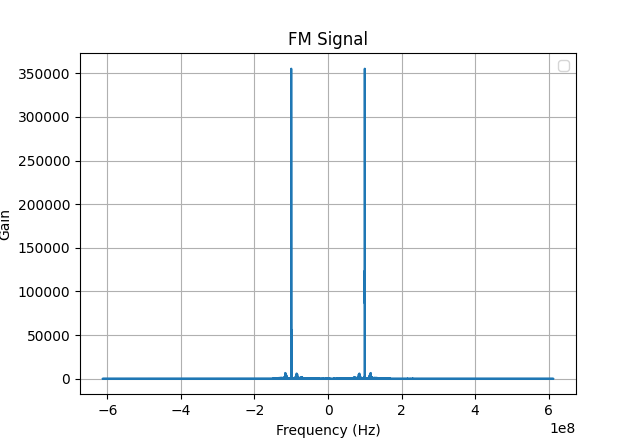
\includegraphics[width=\columnwidth]{fm.png} 
\caption{spectrum analysis of fm signal}
\label{fig:fm_spectrum}
\end{figure}

The spectrum of FM signal is plotted in \figref{fig:fm_spectrum} using below code
\begin{center}
\fcolorbox{red}{white}{\parbox{7.5cm}
{\href{https://github.com/KrishnaYadati/signal-processing/tree/main/fm/codes/mod.py}
{/codes/mod.py}}}
\end{center}


\item Calculate the bandwidth of the transmitted signal by computing the Fourier Transform:
\begin{equation}
S_k = \sum_{n=0}^{N-1} s(n) e^{-j2\pi kn/N}, \quad k=0,1,\dots,N-1
\end{equation}
In code for computing the FFT of s(n)
\begin{equation}
S_k = \texttt{fft}(s(n), N)
\end{equation}
Where $S_k$ is the frequency representation of the signal, s(n) is the transmitted signal. 
we need to calculate its power spectral density. This can be done using the equation \eqref{eq:psd}

Calculating the Power Spectral Density: 
\begin{align}
PSD(s)=\lvert S_k \rvert^2 
\label{eq:psd}
\end{align}
Identify the frequency range with significant power using a mask function. 

\end{enumerate}
\section{\textbf{Demodulation:}}
To demodulate the FM signal and recover the original message signal, we can use the following steps:\\
\begin{figure}
\tikzstyle{block} = [rectangle, draw, fill=white!20, text width=5em, text centered, rounded corners, minimum height=4em]
\tikzstyle{line} = [draw, -latex']
\hspace{-1cm}
\begin{tikzpicture}[ node distance=3 cm, auto]
    % block
      \node[block] (a) {$A_c$ cos(2$\pi$ $f_c$t+2$\pi$ $K_f$ $\int m(T)dT$)};  
     \node[circle, draw,right= 2cm of a] (b) {X}; % these are the name of the blocks 
    \node [block, above of=b] (g){$A_c$cos(2$\pi$f$_{c}$t)};
      \node [block,right of= b] (c) {Low Pass Filter};  
      \node [block,below of = c] (d) {Inverse Cosine};
        \node [block, left of=d ] (e){Differentiator};
       \node [block, left of=e ] (f){$m_1(t)$ };
        
     %line   

%\path[line, shorten >= 1.8cm] (a) -- (b); % adjust the length of the arrow using shorten >=



    \path[line] (a) -- (b);
    \path [line] (b) -- (c);
    \path [line] (c) -- (d);
    \path [line] (d) -- (e);
     \path [line] (e) -- (f);
    \path [line]  (g) -- (b);
    
 \end{tikzpicture}
\captionof{figure}{FM Receiver Block Diagram }
\label{fig:rx_blk}
\end{figure}



\begin{enumerate}
 \item    Multiply the FM signal $s(t)$ with a local oscillator signal $A_c\cos(2\pi F_ct)$. This gives us:
 \begin{align}   
    s(t)*c(t)& = A_c \cos(2 \pi F_c t )*  A_c \cos (2 \pi F_c t +2\pi K_{f} \int_{0}^t m(\tau) d\tau) \\
    \begin{split}
    &=\frac{{A_c}^2}{2}[\cos (4 \pi F_c t +2\pi K_{f} \int_{0}^t m(\tau) d\tau)\\ & + \cos (2\pi K_{f} \int_{0}^t m(\tau) d\tau))]  
    \end{split}
    \end{align}
    
    \begin{figure}
\centering 
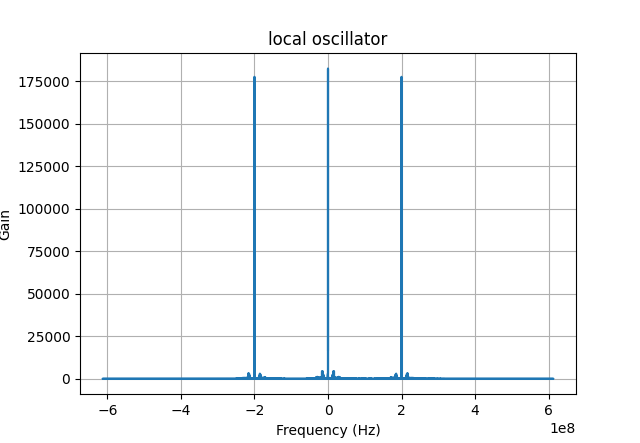
\includegraphics[width=\columnwidth]{lo.png} 
\caption{local oscillator}
\label{fig:lo}
\end{figure}

\item    Pass the result through a low-pass filter to remove the higher frequency components and extract the lower sideband. The resulting signal can be expressed as:
    \begin{align*}
     v(t)=\frac{{A_c}^2}{2}\cos (2\pi K_{f} \int_{0}^t m(\tau) d\tau)
    \end{align*}
    \begin{figure}
\centering 
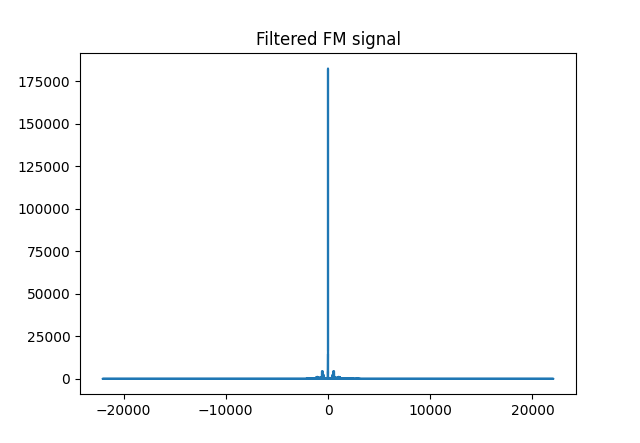
\includegraphics[width=\columnwidth]{lp.png} 
\caption{Filtered signal}
\label{fig:LPF}
\end{figure}
\item  The filtered Signal is then expressed in terms of invese cosin
  \begin{align*}
  {V_1}(t)&=\cos^1(v(t))\\
  &=\frac{{A_c}^2}{2}\cos^1(\cos (2\pi K_{f} \int_{0}^t m(\tau) d\tau))\\
  &={A_c}^2\pi K_{f} \int_{0}^t m(\tau) d\tau)
  \end{align*}


 \item   To recover the original message signal, we can differentiate the signal $V_1(t)$ with respect to time. This gives us:
\begin{align}
m_1(t)&= \,d/dxV_1(t)\\
&={A_c}^2\pi K_{f} \,d/dx \int_{0}^t m(\tau) d\tau)\\
&=A * m(t)
\end{align}

where A=${A_c}^2\pi K_{f}$

\begin{figure}
\centering 
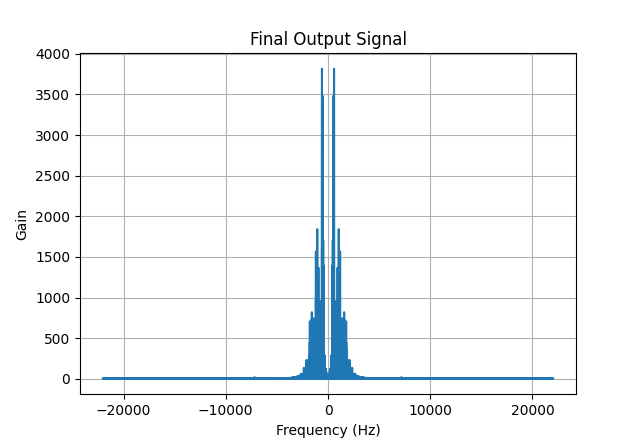
\includegraphics[width=\columnwidth]{./final.png}
\caption{Recovered message signal}
\label{fig:final}
\end{figure}
\end{enumerate}

In code calculates the derivative of the signal $V_1(t)$ using a finite difference method. In particular, it uses the forward difference approximation, where the derivative of a function $V_1(t)$ at point t is approximated as:
\begin{align}
V'(t) \approx \frac{V(t+\Delta t) - V(t)}{\Delta t}
\end{align}

 where ${\Delta t}$  is a small increment. In the code, ${\Delta t}$ is taken as the difference between successive time points t[i+1] - t[i].
 The resulting array $m_1(t)$  contains  the derivative of $V_1(t)$ at each point in t.

\section{\textbf{Result}}

  Upload an audio signal , converting the audio signal into a modulated signal using FM modulation,  and demodulating the signal to retrieve the original audio signal using python.\figref{fig:final} shows the spectrum of demodulated signal. The retrieved audio signal can be saved as a file or played back in real-time using Python.

\begin{center}
\fcolorbox{red}{white}{\parbox{7.5cm}
{\href{https://github.com/KrishnaYadati/signal-processing/tree/main/fm/codes/fm.py}
{/codes/fm.py}}}
\end{center}


\end{document}